\subsection{Esercizio 22}
Sappiamo che $k = (b-a)$ e $k_n=(b-a)\frac{1}{n}\sum_{i=0}^{n}\abs{c_{in}}$. Il rapporto sarà dunque dato da: \[\dfrac{k_n}{k} = 
\dfrac{(b-a)\frac{1}{n}\sum_{i=0}^{n}\abs{c_{in}}}{b-a} = \frac{1}{n}\sum_{i=0}^{n}\abs{c_{in}} \]
Calcolando il rapporto per $n = 1,.....,50$ si ottiene:\\\\
    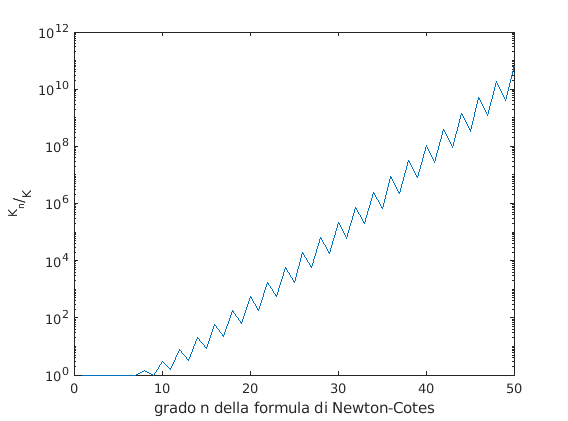
\includegraphics[scale = 0.7]{capitolo5/ncotes.png}

